%% This is file `elsarticle-template-1-num.tex',
%%
%% Copyright 2009 Elsevier Ltd
%%
%% This file is part of the 'Elsarticle Bundle'.
%% ---------------------------------------------
%%
%% It may be distributed under the conditions of the LaTeX Project Public
%% License, either version 1.2 of this license or (at your option) any
%% later version.  The latest version of this license is in
%%    http://www.latex-project.org/lppl.txt
%% and version 1.2 or later is part of all distributions of LaTeX
%% version 1999/12/01 or later.
%%
%% Template article for Elsevier's document class `elsarticle'
%% with numbered style bibliographic references
%%
%% $Id: elsarticle-template-1-num.tex 149 2009-10-08 05:01:15Z rishi $
%% $URL: http://lenova.river-valley.com/svn/elsbst/trunk/elsarticle-template-1-num.tex $
%%
\documentclass[preprint,12pt]{elsarticle}

%% Use the option review to obtain double line spacing
%% \documentclass[preprint,review,12pt]{elsarticle}

%% Use the options 1p,twocolumn; 3p; 3p,twocolumn; 5p; or 5p,twocolumn
%% for a journal layout:
%% \documentclass[final,1p,times]{elsarticle}
%% \documentclass[final,1p,times,twocolumn]{elsarticle}
%% \documentclass[final,3p,times]{elsarticle}
%% \documentclass[final,3p,times,twocolumn]{elsarticle}
%% \documentclass[final,5p,times]{elsarticle}
%% \documentclass[final,5p,times,twocolumn]{elsarticle}

%% The graphicx package provides the includegraphics command.
\usepackage{graphicx}
\graphicspath{ {./images/} }
%% The amssymb package provides various useful mathematical symbols
\usepackage{amssymb}
\usepackage{amsmath}
%% The amsthm package provides extended theorem environments
%% \usepackage{amsthm}

%% The lineno packages adds line numbers. Start line numbering with
%% \begin{linenumbers}, end it with \end{linenumbers}. Or switch it on
%% for the whole article with \linenumbers after \end{frontmatter}.
\usepackage{lineno}

%% natbib.sty is loaded by default. However, natbib options can be
%% provided with \biboptions{...} command. Following options are
%% valid:

%%   round  -  round parentheses are used (default)
%%   square -  square brackets are used   [option]
%%   curly  -  curly braces are used      {option}
%%   angle  -  angle brackets are used    <option>
%%   semicolon  -  multiple citations separated by semi-colon
%%   colon  - same as semicolon, an earlier confusion
%%   comma  -  separated by comma
%%   numbers-  selects numerical citations
%%   super  -  numerical citations as superscripts
%%   sort   -  sorts multiple citations according to order in ref. list
%%   sort&compress   -  like sort, but also compresses numerical citations
%%   compress - compresses without sorting
%%
%% \biboptions{comma,round}

% \biboptions{}

\usepackage[utf8]{inputenc}
\usepackage[english]{babel}
%%\usepackage[demo]{graphicx}
%%\usepackage{babel,blindtext} 

\usepackage{xcolor}

\journal{Journal Name}

\begin{document}

\begin{frontmatter}

%% Title, authors and addresses

\title{Proteinas Canijas}

%% use the tnoteref command within \title for footnotes;
%% use the tnotetext command for the associated footnote;
%% use the fnref command within \author or \address for footnotes;
%% use the fntext command for the associated footnote;
%% use the corref command within \author for corresponding author footnotes;
%% use the cortext command for the associated footnote;
%% use the ead command for the email address,
%% and the form \ead[url] for the home page:
%%
%% \title{Title\tnoteref{label1}}
%% \tnotetext[label1]{}
%% \author{Name\corref{cor1}\fnref{label2}}
%% \ead{email address}
%% \ead[url]{home page}
%% \fntext[label2]{}
%% \cortext[cor1]{}
%% \address{Address\fnref{label3}}
%% \fntext[label3]{}


%% use optional labels to link authors explicitly to addresses:
%% \author[label1,label2]{<author name>}
%% \address[label1]{<address>}
%% \address[label2]{<address>}

\author[1]{Ale Zavala}
\author[1]{Sergio Hern\'andez }
\author[1]{Pedro Miramontes}
\author[2]{León Martínez}

\address[1]{Facultad de Ciencias, National Autonomous University of Mexico, Mexico City 04510, Mexico}
\address[2]{Metropolitan Autonomous University}

\begin{abstract}
%% Text of abstract
¿Qué proponemos como abstract?
\end{abstract}

\begin{keyword}
Intrinsically disordered protein regions \sep ordered protein regions \sep Pfam family \sep protein domain \sep The discrete generalized beta distribution \sep megasecuence \sep familiome \sep self-organizing map \sep complexity
%% keywords here, in the form: keyword \sep keyword

%% MSC codes here, in the form: \MSC code \sep code
%% or \MSC[2008] code \sep code (2000 is the default)

\end{keyword}

\end{frontmatter}

%%
%% Start line numbering here if you want
%%
\linenumbers

%% main text
\section{Background}
\label{S:1}

\par NOTA: HAY QUE CONSIDERAR QUE LA REVISTA A LA QUE SE VA A ENVIAR ES Computational Biology and Chemistry de Elsevier. \par PARTE DE LA INTRODUCCIÓN SE DEBE QUITAR C0NSIDERANDO QUE MUCHOS DE LOS LECTORES SABRÁN ACERCA DE PROTEÍNAS Y PUEDEN SER HASTA BIOINFORMÁTICOS. \par


Historically, the science of protein structure has privileged the study of ordered protein regions (OPRs)  with regular and well-defined secondary structure, such as  $\alpha$-helix, $\beta$-conformations and turns. In fact, proteins that contain mainly ordered regions are the classic text-book example of what a typical protein should look like. This is probably associated with the fact that the most commonly used technique for determining protein structure, i. e. x-ray crystallography, is biased towards resolving protein regions with regular and well-defined secondary structures. However,  it has recently become increasingly clear that intrinsically disordered protein regions play an important role in the structure of proteins \cite{oldfield2014intrinsically}.

Intrinsically disordered protein regions (IDPRs), are segments of polypeptides, that do not natively acquire well defined, regular, or repetitive, secondary structures and instead adopt many different structural ensembles with no single, preferred lowest energy conformation and have biological activities that are dependent on this disordered state. There are some computational tools that can predict the order/disorder state of a protein region using only the complete polypeptide sequence as input \cite{vucetic2004disprot},  \cite{piovesan2016disprot}. IDPRs have been found to be prevalent in eukaryotes and are common in bacteria and archaea too (XXX?  ¿PEDRO: que significa esta nota?)  \cite{dunker2000intrinsic} \cite{dunker2002intrinsic} \cite{dunker2013s} \cite{oldfield2014intrinsically}. A general function that has been proposed for many IDPRs is the binding to other molecules, including proteins, nucleic acids and other ligands \cite{dunker2001intrinsically} \cite{van2014classification} \cite{oldfield2014intrinsically}. However, it is possible that the importance of IDPRs goes beyond this currently accepted function, and that they may even play an important role in the folding and functioning of proteins. We would like to emphasize that in this study we have tried to jointly analyze both the OPRs and IDPRs. This approach derives from our belief that at least some of the properties of proteins are the product of the interactions between OPRs and IDPRs. Furthermore, we hypothesize that the distribution pattern of OPRs and IDPRs within a given protein domain is specific to that domain  (similar to a fingerprint) and also specific to that domain’s family. We will expand on the definition of protein families and other related concepts in the following sections. 

Here, we will only mention that studying patterns of protein order/disorder at the level protein domains (instead of single proteins) allowed us to capture amino acid sequence variability that was, in principle, compatible with the tertiary structure conservation that characterizes a domain. Additionally, each representative of a domain acted as a new quasi-replicate thereof, allowing us to (naturally) increase the sample size of the data series to be analyzed with our proposed statistical tools (see below). Furthermore, we augmented our protein sequence data with gene ontology (GO) annotations in order to explore whether functional information of protein domains correlates with their order/disorder regularities. 

Measures of complexity of patterns of OPRs and IDPRs have the potential to contain information on structural and functional aspects of proteins in the sense that members of a given protein family that are close to each other in the parameter space of some measures of complexity could also be close in terms of functional properties. If IDPRs are an integral part of proteins the patterns of alternating OPRs and IDPRs of varying lengths should be relatively conserved among members of a protein family. Potentially, measures of the complexity of such patterns could capture enough information thereof, such that they could serve as a proxy for characterizing specific proteins.

In this study we will use several measures of complexity of a polypeptide pattern. At this time "complexity" can be understood as how close or how far a sequences is from two extremes: randomness or periodicity. On one hand, he well known Kolmogorov’s complexity index (K) provides a measure of how far a sequence is from being random and, on the other,  Shannon’s entropy (H) tells us how far is a sequence from the equiprobable distribution (REFSXXX). Additionally, the recently proposed Discrete Generalized Beta function (DGBF)  of rank-ordered distributions has also emerged as a measure of complexity. Interestingly, the DGBF can separate intermittent regimes from chaotic dynamics and may serve as an indicator of transitions between these two regimes in a wide array of phenomena \cite{martinez2009universality}.

Here, we propose  the use of the above mentioned descriptors to place any given protein into a space of parameters and to discuss they way different families of proteins group in such a space. Our working model will be the Saccharomyces cerevisae proteome. We discuss the possibility that the DGBF of patterns of protein order/disorder may be able to detect evolutionary transitions in which ordered proteins acquire or expand their disordered regions or in which disordered protein start to limit their conformational repertoires. 



\bigbreak
\begin{itemize}
\item \color{red}
\textbf{Esta parte la va a “arreglar Pedro”.}
\bigbreak
with affinities to other phenomenological descriptions such as power laws, that is able to capture the “flavor” of a given complex system and differentiate it from other similar yet distinguishable systems, while at the same time being robust to the finite size effects that often affect power law descriptions of physical phenomena. 
\end{itemize}

\bigbreak

Here, we propose  to use a discrete version of the generalized beta function as well as Kolmogorov K and Shannon H as descriptors of the order-disorder patterns of protein domains present in the Saccharomyces cerevisiae “familiome” (a novel concept that we propose and that refers to the complement of Pfam families present in the baker’s yeast a proteome).



\bigbreak

\bigbreak

\begin{itemize}
\item 
\color{red}
\textbf{M{\'A}S DE QUE ESPERAMOS}
R:.
\bigbreak

Idea 1.
En este art{\'i}culo utilizamos un m{\'e}todo novedoso nunca antes aplicado en el {\'a}rea de la estructura de las prote{\'i}nas denominado germibeta. Nuestra hip{\'o}tesis es que obtendremos una combinaci{\'o}n de valores espec{\'i}fica e independiente para cada familia a partir de la entrop{\'i}a, la complejidad algor{\'i}tmica y la funci{\'o}n beta caracter{\'i}stica de sus patrones de orden-desorden que esperamos pueda servir como un nuevo atributo para caracterizar a una familia de prote{\'i}nas.

\bigbreak

Si lo anterior no se cumple, idea 2:
En este art{\'i}culo utilizamos un m{\'e}todo novedoso nunca antes aplicado en el {\'a}rea de la estructura de las prote{\'i}nas denominado germibeta. Este m{\'e}todo nos ayudar{\'a} a entender (aqu{\'i} no sabemos qu{\'e} es exactamente lo que nos ayudar{\'a} a entender) que junto con el proceso biol{\'o}gico de la estructura de las prote{\'i}nas permiten aumentar el conocimiento de la funci{\'o}n de las mismas en base al estudio de las RIDs/ROs.
Palabras clave: describir, caracterizar, dominio, prote{\'i}nas, propiedades de las familias o proteínas o dominios. 
\end{itemize}




\bigbreak



\section{Materials and Methods}
\label{S:1}

\subsection{Construction of the database of complete sequences represented in the yeast familiome}

In this study, our aim is to characterize protein families in terms of the entropy, algorithmic complexity and characteristic beta function of their order-disorder pattern. A family of proteins is  a group of proteins or  protein domains that share patterns of significant sequence conservation, due to common ancestry, that frequently entail functional similarity \cite{nelson2017lehninger}. A protein domain is a substructure produced by any contiguous part of a polypeptide chain whose structural features are independent of the rest of the protein. A domain usually contains between 40 to 350 amino acids, and it is the modular unit from which many larger proteins are constructed \cite{alberts2015molecular}. It is important to note that any given protein does not necessarily belong to a single family, as a given protein can contain several domains with different evolutionary histories, and indeed, many proteins belong to several families \cite{bateman1999pfam}. Although most protein domains that are identified using sequence-based approaches are have well-defined and relatively stable spatial structures, some can be fully or largely disordered or can contain conserved disordered regions \cite{xue2010pondr}, these are known as intrinsically disordered domains (IDDs; \cite{tompa2009close}).
The protein families information is provided by the Pfam database \citet{sonnhammer1997pfam} \cite{bateman2004pfam} \cite{punta2011pfam} \cite{finn2015pfam}. Pfam is a collection of protein domains and protein families in which each family is represented by two multiple sequence aligments and two profile-Hidden Markov Models, one of the two alignments is a high quality seed alignment \cite{sonnhammer1997pfam} \cite{bateman2004pfam}.

To build our yeast familiome database, we explored protein information in several biological databases. To every translated gene from Saccharomyces Genome Database (v2015; https://www.yeastgenome.org/; \cite{cherry2012saccharomyces}) we associated an UniProt identifier and its complete polypeptide sequence (“uniprot” full file, v2014; \cite{gene2015gene}). Using the UniProt information, we linked to every yeast protein its corresponding  Pfam families (v28, 2015; https://pfam.xfam.org/;  \cite{bateman1999pfam}  \cite{punta2011pfam}). Subsequently, for each Pfam family from S. cerevisiae familiome we downloaded its Pfam-A seed alignment file (v28, 2015; \cite{sonnhammer1997pfam} \cite{punta2011pfam} (XXXXXXXX ?) , which contains only the aligned segments that belong to a protein family of a variety of species. Finally, we used the UniProt identifier provided by the Pfam-A seed alignment file and the UniProt full file to obtain the complete polypeptide sequence of each protein in the Pfam-A seed alignments of the yeast familiome. 



\subsection{Predicting intrinsically disordered residues in each polypeptide sequence of yeast familiome}

In order to assign each residue from our complete polypeptide sequence yeast familiome database to either the “ordered” or “intrinsically disordered” categories we used the open-source DisEMBL prediction software. DisEMBL is  based on artificial neural networks trained to predict three different definitions of disorder and displays  the disordered segments of arbitrary length within a protein sequence \cite{linding2003protein}. We used the three differents algorithms of DisEMBL: loops/coils, hot loops and remark465 and the final assignment of each residue as either ordered  or  disordered residue  was based on a majority rule decision between the three predictions. The order/disorder information was coded into the sequences as UPPERCASE/lowercase one-letter amino acid symbols, respectively. This procedure was performed for each complete polypeptide sequence of each Pfam-A seed alignment family in the yeast familiome. All the members in one family were concatenated together into one big megasequence.
 

\subsection{Transferring the ordered/disordered information to the Pfam-A families seed alignment}

In our study, we needed to associate sequences of the Pfam-A families seed alignment of the yeast familiome with the DisEMBL majority rule decision results. In order to do this we used options of the MAFFT program to maintain the Pfam-A families seed alignment unchanged, to maintain the gaps, the UPPERCASE/lowercase in the alignment and to preserve intact the order of the residues \cite{katoh2012adding} \cite{katoh2012adding} in the Pfam-A families seed alignment of the yeast familiome.  


\subsection{Gene Ontology annotations in the yeast familiome}

To enrich our yeast familiome database, for those Pfam families where this information was available, we associated the molecular function annotation from Gene Ontology (v2018; http://geneontology.org/; \cite{ashburner2000gene} \cite{gene2015gene}). We needed a general molecular function annotation so we manually curated the specific GO molecular function annotations of the yeast familiome.


\subsection{Megasequence construction}
In order to have a sequence big enough to statistically represent the whole family in a robust way, we constructed what we called a megasequence which consisted in all the domain instances within a family glued together, so the statistical regularities will be magnified and easily observable in the so called megasequence.

We took all the aligned sequences for a given domain and spliced them one after another to obtain a family megasequence.

\subsection{The discrete generalized beta distribution (DGBD)}

All these megasequences of the yeast familiome were compared using a discrete generalized beta distribution (DGBD) \cite{martinez2009universality} \cite{petersen2011statistical} which is a rank ordering distribution that takes the form:

\[
f(r) = \dfrac{A(N+1-r)b}{r^a}  
\]

Where a and b are parameters to be found, N is the number of ranks and A is a normalization constant. This rank ordering distribution has been successfully used across a wide range of different phenomena regardless of the truncated scaling behavior shown typically in most of the rank-order distributions.
The approach used in our analysis is as follows. We took all the aligned sequences and merge them together one after another to make a family megasequence, then we counted the frequencies of the different words of length 2 and ordered these distributions of sizes in decreasing order. Then, through a nonlinear fit of (1) we obtained the (a,b) pair which was used to represent the distribution. 

\subsection{Shannon Entropy (H(X))}
Another attribute added to the whole yeast familiome was the calculation of Shannon’s Entropy for each of the sequences of the larger. Shannon’s Entropy is defined as follows:

\[
H(X) = \sum{ \dfrac{p\_i}{log(p\_i)}}       (2)
\]

Where p\_i is the probability of one of the N amino acids in the megasequence X. Applying H(X) to every family megasequence we have will reveal which sequences are the furthest from the normal distribution and so, which megasequence has the most structure in it \cite{alberts1925adami}.

\subsection{Kolmogorov complexity}

Kolmogorov complexity index when applied to a string of characters, in our case is the megasequence X, can be interpreted as the complexity of a computer program required to reproduce megasequence X. The calculation of Kolmogorov’s complexity index can be approximated as follows:

\[
k(seq) = {\dfrac{length(compressed(seq))}{length(seq)}} (3)
\]

Where seq is the original megasequence of some family of proteins. The actual implementation of this function was done in Python computer language where zlib libraries were used to compress every sequence of the familiome \cite{li1989kolmogorov}.
In our experiment we used K as another attribute together with the already described, in order to understand the algorithmic complexity assumed to exist in every family. That is, if a set of instructions is behind the description of every protein in each family, we would expect that K captures this particular complexity.


\subsection{Self-organizing map}

The self-organizing map (SOM) is an unsupervised neural network used for data analysis and dimensionality reduction \cite{kohonen2013essentials}. It has been long being applied into data analysis and biological sciences to detect similar profiles of analyzed data \cite{wang2002clustering, nurminen2018impact}. The basic algorithm is divided in two steps. First, an initial map is formed with N neurons arranged in a lattice which will represent M d-dimensional vectors. Each of the N neurons contains a single d-dimensional prototype that will be modified during the training of the map. Then, for each vector sample a winning prototype must be found. The second step consists in modifying the prototypes of all vectors within a neighborhood of this winning neuron, the magnitude of the modification is in proportion to the distance of the winning neuron. This process ends up unfolding a map where each prototype in neurons represents local averages of data, hence nearby neurons have similar prototypes.
Once the SOM is formed, locally grouped families must be assigned to a group. This step is done by a hierarchical clustering using euclidean distance. The number of groups was determined by the Davies-Bouldin index.


\section{Results}
\label{S:1}

\subsection{Saccharomyces cerevisiae familiome database}



\bigbreak
Our yeast familiome database contains 538 Pfam families (protein domains) and a total of NNNN instances of domains. The size range of the families goes from a family containing XXXX instances of a domain (Family number PF????) to a family containing YYYY instances (Family PF¿¿¿¿) All instances of a given domain were concatenated to obtain a megasequence, thus yielding a total of 538 megasequences. Each megasequence contains information of ordered/disordered status for all its residues, as well as the values of the parameters $\alpha$ and $\beta$ from the expression of DGBD, Shannon's entropy, and Kolmogorov complexity. Additionally, for 260 families we have the specific GO molecular function corresponding to 18 different GO categories namely hydrolase, electron transfer activity, protein dimerization activity, isomerase, motor activity, transferase, transmembrane transporter, translation initiation factor activity, binding, translocases, antioxidant activity, structural constituent, oxidoreductase, ligase, structural molecule activity, catalytic activity, lyase, and copper chaperone activity. This information is shown in supplementary material S1-Yeast Familiome.

\bigbreak



\subsection{Using a discrete version of the generalized beta function to classified {\it S. cerevisiae} familiome}
With regard to the meaning of the DGBD parameters, in some instances the exponent a can be related to behaviors generating power laws, as is the case of scale invariance in turbulence in the so called inertial range where energy is transferred between different scales at the same rate, while b seems to be associated with chaotic, disordered fluctuations, for example the dissipative range for turbulence. The DGBD manages to encompass both types of regimes as well as their crossover. Further understanding of the exponents comes from our expansion-modification study where a conflicting dynamics leads to the DGBD. The expansion component which preserves a given trend is associated with a, on the other hand the modification part favors change and is related to b. Though we have shown that these conflicting permanence-change processes can produce DGBD, we are in no position to consider them as a requirement. On occasions we have perceived that parameters relations hold for certain instances, for example the for the musical notes frequencies $\alpha < \beta$ in general, while for network connectivity related situations $\alpha > \beta $ is encountered more often. However, the role of exponents a and b as universality classifying parameters, as for example in critical phenomena, remains be investigated in further detail. Our findings are most revealing when both parameters a and b are non-negligible and not too disparate. This usually happens for the social phenomena we have explored and which present some the most impressive fits. Based on these examples, it appears that DGBD fits are at their best when dealing with situations that result from the convergence of multiple heterogeneous processes. \cite{martinez2009universality}. \par EL PÁRRAFO ANTERIOR ES INTEGRO DEL ARTÍCULO DE MARTÍNEZ-MEKLER Y ES PARA AYUDARNOS A TRATAR DE RESPONDER LAS SIGUIENTES DUDAS.... \par Idea del día 12 de abril del 2021. Describir la ley de potencia y las ventajas que confiere la germibeta. Hacer énfasis en que la megasecuencia de las familias se ajusta perfectamente a la forma de la germibeta tanto en alfa como en beta (A Alejandra le parece fundamental este punto). Los ajustes de la germibeta se pueden utilizar para "buscar" o "identificar" o "interpetar" las RIDs/ROs (Si esto es verdad, aquí puede quedar el argumento de la estructura de las proteínas integrando las RIDs/ROs como parte del todo de la proteína, indicar si esto también es valido para que las RIDs/ROs sean una huella digital, todavía no estamos seguros si la huella digital puede ser evolutiva también).  \par ESPECIFICAR PARA QUE SE HICIERON CADA UNA DE LAS FIGURAS.... QUÉ SE QUERÍA OBTENER... QUÉ RESULTADOS IMPORTANTES SE TIENEN Y EN BASE A QUÉ.... \par  We constructed DGBD plots for the 580  families and we are showing the best DGBD plots according to the following criteria: first, a Pfam family needed to have the highest square of correlation coefficient; second, an sample size N of at least  30 different domain instances; and finally the DGBD alpha and beta values had to be $\ge 0$. Every panel in each figure indicates the Pfam family, the square of correlation coefficient, the alpha and beta values, and its N value. \par In the familiome database, the highest alpha value was 2.0027 and the lowest alpha value was 0.1003. Figure 1 shows selected cases for the scenario where $ \alpha > \beta$.  In this database, we have the best 30 DGBD graphs with high alpha and low beta values and there are 5 different general GO molecular functions belonging to 11 different Pfam families. Seven of these eleven have a ``binding'' GO, 2 have ``ligase'' GO and ``oxidoreductase'', ``isomerase'' and ``lyase'' ontologies have one each (Figure 1). Althought there are seven general binding ontologies, we cannot group them because their specific ontologies are different. We have two ``protein binding'' ,  one ``ATP binding'',  one ``thiamine binding'', one ``DNA binding'', one ``metal ion binding'', and one ``phosphatidylinositol binding''. For ligase ontology, we have two different Pfam families with specific ontologies like ``aminoacyl-tRNA ligase'' activity and ``aminoacyl-tRNA editing'' activity. In the case of a family with lyase ontology, its specific ontology is ``phosphatidylserine decarboxylase activity''. For the families with oxidoreductase and isomerase, there are not specific ontologies. 
These phenomena are encountered more often for network connectivity related situations $\alpha > \beta$ \cite{martinez2009universality}. ESTA FRASE LA SUGIRIÓ CHEKO PERO PARECE QUE ESTÁ INCOMPLETA ¿A QUÉ TE REFIERES CON REDES DE CONECTIVIDAD? ¿REDES LIBRES DE ESCALA?¿REDES CON CONECTIVIDAD ALTA O BAJA? ¿REDES CON DETERMINADOS GRADOS DE LIBERTAD? ADEMÁS ¿CÓMO SE CONECTA ESTO CON LA DISCUSIÓN?




\begin{figure} %{\textwidth}
    \centering
    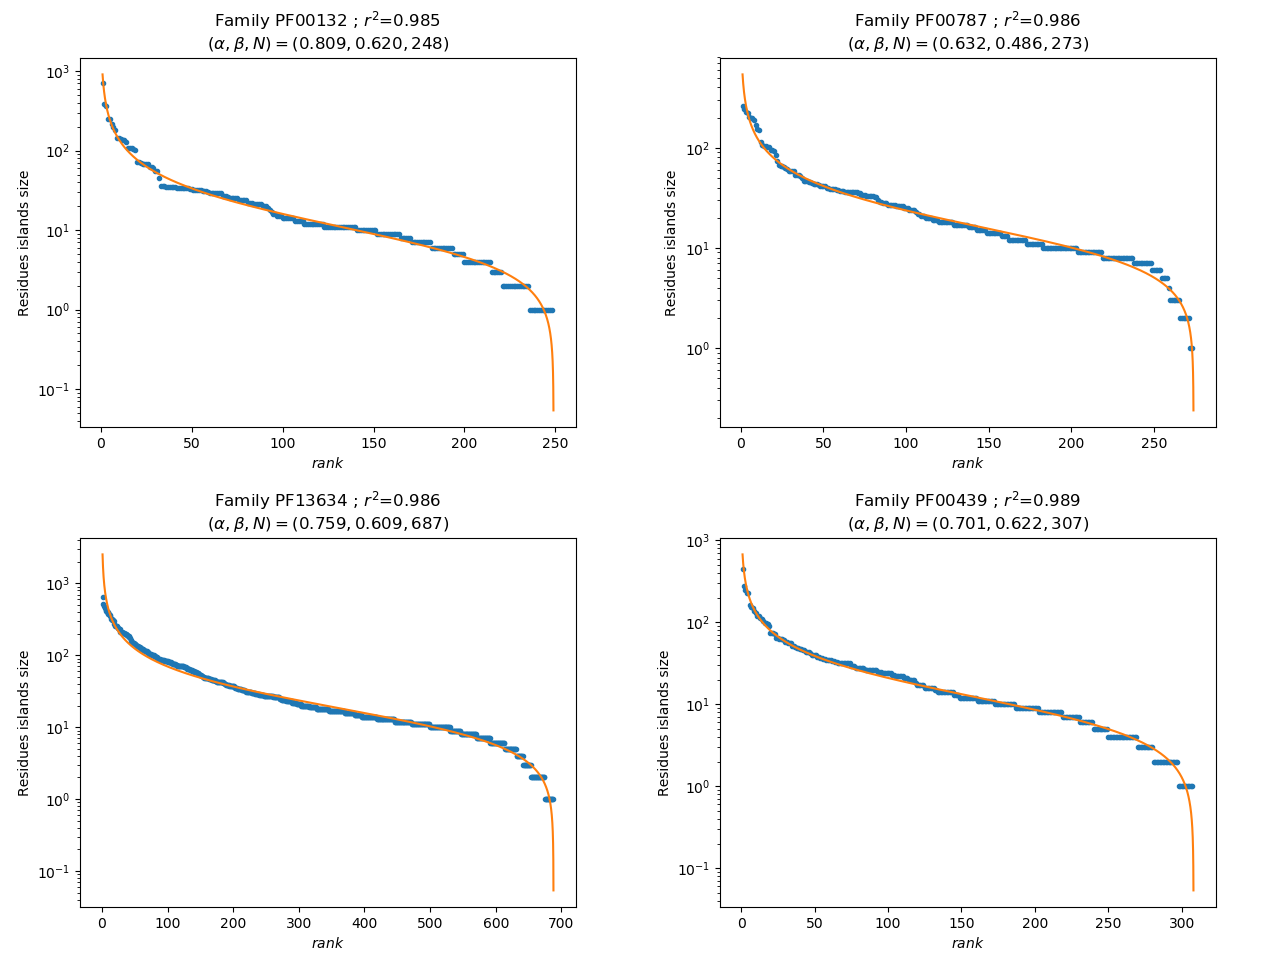
\includegraphics[width=13cm]{images/01_mejoresAlfa.png}
    \caption{Semilog DGBD plots with high $\alpha$ and low $\beta$ values.  Orange lines represent  the best fitting DGBD model for the corresponding experimental data points (shown in blue). Values for the $\alpha$ and $\beta$ parameters of the DGBD as well as sample size are shown on top of each panel. PF00787 and PF00439 families have binding molecular function ontology, whereas PF00132 and PF13634 do not have an assigned GO. Notice that  x- and y-axis scales are different among panels.}
    \label{fig:alpha}
\end{figure}
\clearpage


In the yeast familiome database, the highest beta value was 1.6529 and the lowest beta value was 0.0236. Figure 2 show the cases in which $\alpha < \beta $, namely  4 from among the best 30 DGBD graphs with high beta and low alpha values. There can be found 5 different general GO molecular functions associated  with different families. Seven families have ``binding'' ontology, whereas ``transferase'', ``translocase'', and ``ligase'' are found in only one family each (Figure 2). Although the binding function  has a clearly higher prevalence, we have 9 different families with different molecular specific binding function. We have 3 families with ``protein binding'' and one family with both ``protein binding'' and ``ATP binding'', two families are labelled ``DNA binding'' and one family is labelled ``DNA binding'' and ``RNA polymerase activity'', one family has ``RNA binding'', one family is labelled ``metal ion binding'', and two families with other specific ontologies like ``proton-transporting ATP synthase activity'' and ``aminoacyl-tRNA editing activity''. In this case, the distribution falls rapidly and with high beta values, the rank is minor in the distribution por lo qué...... 
%\citet{Tesis Cheko}, esto puede estar interesante pero hay que ponerlo con más detalle, o bien explicarnos a los legos la importancia de esta observación, incluso si no tiene una conexión biológica clara, pensamos que la importancia fisico-matemática es importante en sí.
\cite{martinez2009universality}.


\begin{figure} %{\textwidth}
    \centering
    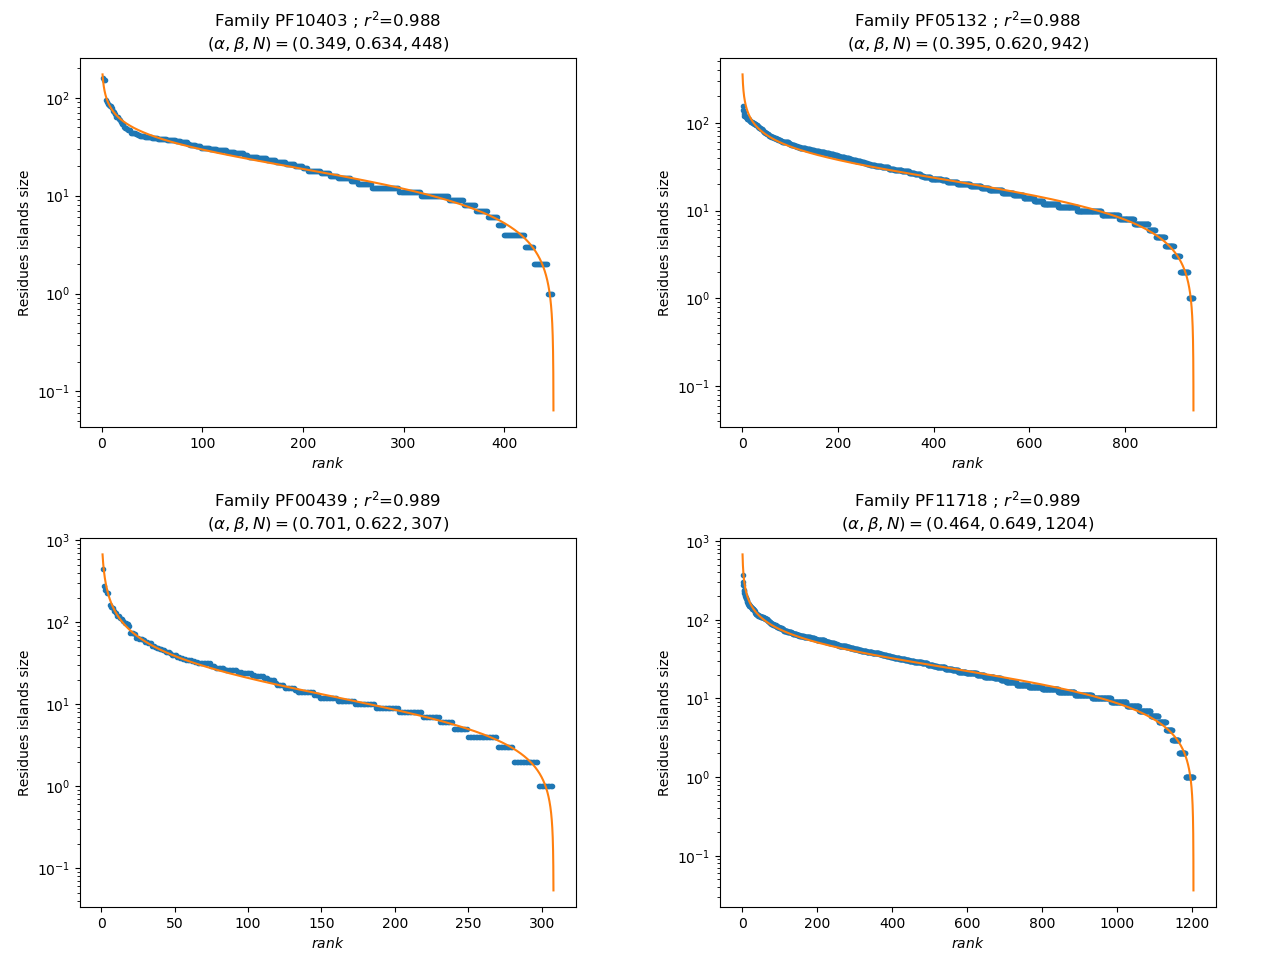
\includegraphics[width=13cm]{images/02_mejoresBeta.png}
    \bigbreak
    \caption {Semilog DGBD plots with high beta and low alpha values. PF05132 family has transferase and binding ontology. PF00439 and PF10403 share binding ontology. Notice that the scales are different.}
    \label{fig:beta}
\end{figure}
\clearpage

\underline{Aquí nos quedamos el 13 deb 2021}. In the yeast familiome database, 28 different families were found when alpha equals beta with values nearest to 1 $\pm0.10$. There are 3 different generals GO molecular functions belonging to different families. Six Pfam families have a binding ontology, two have ligase ontologies, and hydrolase, initiation factor and cooper chaperone ontologies are represented by one each (Figure 3). We have 6 families with different binding ontologies and other ontologies. One family have zinc ion binding and nucleic acid binding, one family have metal ion binding and translation initiation factor activity, one family have ATP binding, nucleotide binding and aminoacyl-tRNA ligase activity, one family have copper ion binding and copper chaperone activity, one family have RNA binding and the last family have ATP-dependent 3'-5' DNA helicase activity and aminoacyl-tRNA editing activity.  \par QUÉ SIGNIFICA ESTO? DISTRIBUCIÓN DE LA VALLETE.... \par

\begin{figure} %{\textwidth}
    \centering
    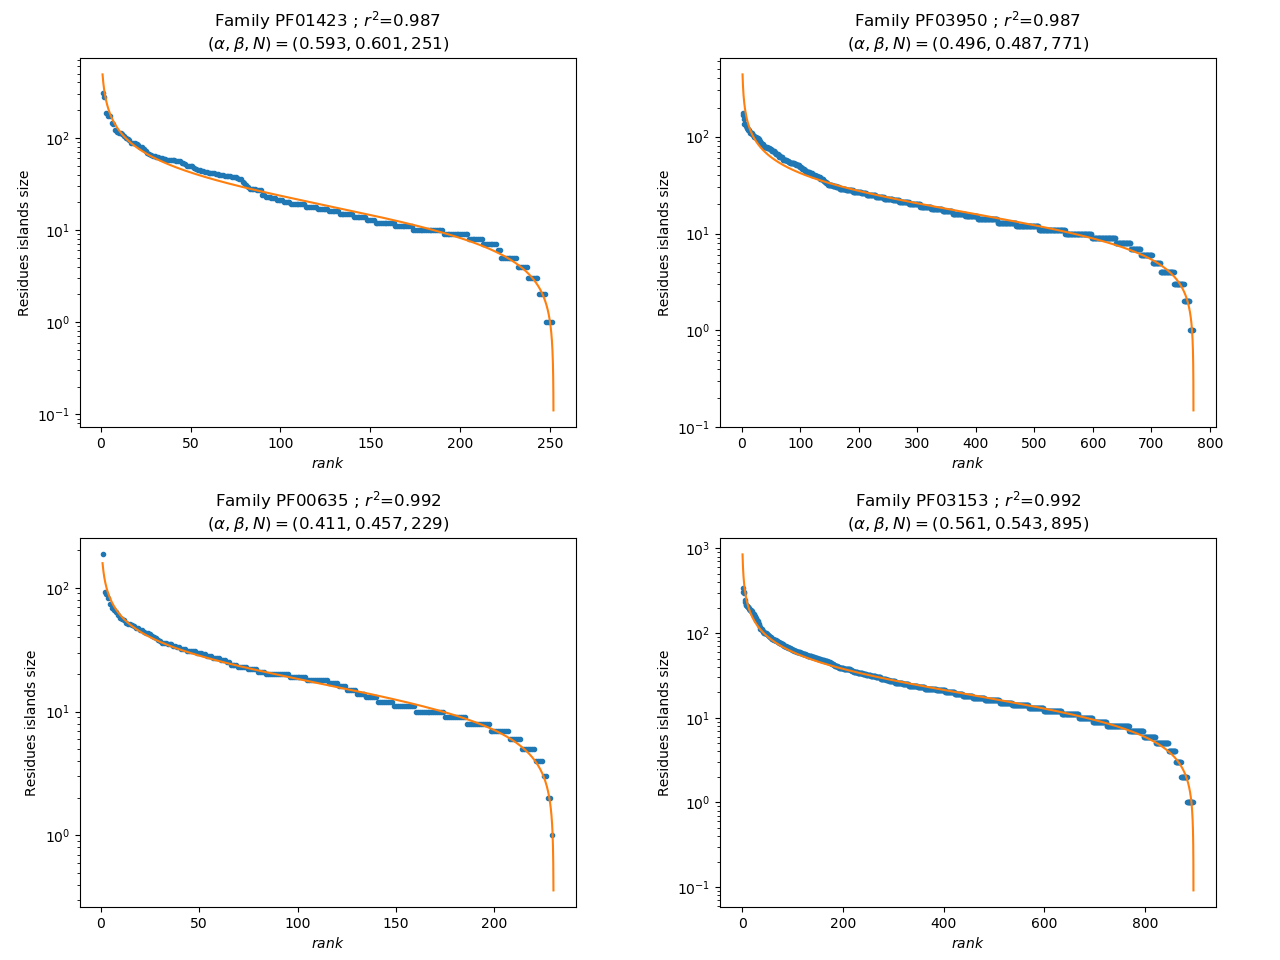
\includegraphics[width=13cm]{images/03_mejoresLaVallete.png}
    \bigbreak
    \caption {Semilog DGBD plots when alpha equals beta. PF03950 has binding and initiating factor ontologies. The scales are different.}
    \label{fig:alphabeta}
\end{figure}
\clearpage


\par DE LAS GRÁFICAS ANTERIORES, CUÁL SERÍA LA DESCRIPCIÓN SERÍA Y FORMAL (FÍSICA)? YO SUPONGO QUE TENIENDO ESA DESCRIPCIÓN PODREMOS DAR UN ANÁLISIS MÁS FORMAL. LO QUE ALEJANDRA HA HECHO ES MERAMENTE DESCRIPTIVO (PAJA). \par
 
In general, the specific ontologies are different between the parameters $\alpha > \beta$, $\alpha < \beta $, and $\alpha = \beta $. There is no consensus in these ontologies, although the three cases are represented by binding and ligase general ontologies. \par LEÓN PATRICIO ENTIENDES LO QUÉ QUIERE DECIR EL PÁRRAFO ANTERIOR? \par


\subsection{\textbf{Self-organizing map.}}

In this work we use a self-organizing map with input data from in a 7-dimensional space. This can be seen in figure 5 and 6 where two maps were constructed using the before mentioned groups of features respectively.  As shown in both of these figures, the lack of a more complex structure like the one shown in figure 4 gives an idea of how the conjunction of both sets of features is required to accomplish such rich structure. Three variables correspond to gene ontology features such as binding, transferase and hydrolase, which are coded in a binary variable whether the attribute is in the family or not. The other four features are: parameters a and b from expression (1),  Shannon’s entropy and Kolmogorv complexity. \par The map was trained with a lattice of 14x14 units. In figure 4 we can see the final map where we can detect 6 groups of clustered families located in the darker blue areas and these patterns and groups cannot be formed neither using gene ontologies  nor the complexity features alone, and in figure 5 we can see in a heatmap each one of different entries of the prototypes, this visualization allows us to see the distribution of the different attributes. In this map all of the 7 attributes were used. From this final figure we can infer that the gene ontology attributes are completely independent from each other. 
\par In figure 4 there are 6 groups of clustered families with different general molecular function annotation between every group and delimited by darker blue areas that are a group of neurons that does not have any family representation. 
The cluster with blue circles have the general molecular function annotation binding. It is the biggest cluster with 93 different families. The molecular function annotation more specific for these families are: protein binding, DNA binding, metal ion binding, ATP binding, RNA binding, nucleic acid binding, thiamine pyrophosphate binding, GTP binding, nucleotide binding, NAD binding, calcium ion binding, heme binding, FMN binding, coenzime binding, flavin adenine dinucleotide binding, phosphatidylinositol binding, pyridoxal phosphate binding, chromatin binding, GTPase binding, ubiquitin binding, iron-sulfur cluster binding, translation binding and histone binding. There are 16 different families from this group that had others molecular function like oxidoreductase, catalytic activity, copper chaperone activity, translation initiation factor activity and protein dimerization activity. The cluster with purple "X" have the general molecular function annotation of transferase and have 26 different families. The molecular function annotation more specific for these families are: phosphotransferase activity, prenyltransferase activity, methyltransferase activity, and others. The red pentagon cluster have the general molecular function annotation of hidrolase and have 22 different families. The molecular function annotation more specific for these families are: endonuclease activity, thiol-dependent ubiquitinyl hydrolase activity, deubiquitinase activity, and others. \par Two clustered families have different molecular functions but join two different groups of clustered families. The yellow plus sign (+) has 8 different families and the molecular function of binding and hydrolase and the dark yellow downward pointing triangles cluster have 7 different families and the molecular function of binding and transferase. These clusters have only these two functions delimited by less dark blue areas and link two big families groups, binding and transferase, and the other families groups are binding and hydrolase. \par Finally, the green square cluster has 49 different families with the rest of the general ontologies that do no has any particular grouping. The ontologies are oxidoreductase, isomerase, ligase, lyase, translocase, transmembrane transporter, structural constituent, catalytic activity, antioxidant activity, structural molecule activity, translation initiation factor activity, motor activity, and electron transfer activity. \par The information in each cluster is different from each one, however, the information in every neuron is very important to clustering one or more families and it has to be direct with the general ontologies and complexity features like DGBD, the Shannon entropy, and the Kolmogorov complexity. In the future, we hope we can predict the family ontology with this kind of result, however, we know that we have to obtain more clear results with this methodology.  


\bigbreak
\par FINALMENTE TRATAR DE DESCRIBIR LAS ZONAS PROHIBIDAS COMO "FACTOR DELIMITANTE". EN ESTE CASO LAS ZONAS PROHIBIDAS SE DESCRIBIERON COMO ZONAS AZULES OSCURAS. \par ES EVIDENTE QUE LA INFORMACIÓN CONTENIDA EN CADA UNA DE LAS ZONAS ES DIFERENTE ENTRE CADA UNA DE ELLAS. APARENTEMENTE LA ONTOLOGÍA EN LAS ZONAS ESTA DOMINANDO, SIN EMBARGO, ES CLARO QUE CADA UNA DE LAS NEURONAS PUEDE CONTENER UNA O MAS FAMILIAS NO SOLO PREDOMINA LA IMPORTANCIA DE LA ONTOLOGÍA SINO QUE LA GERMIBETA, KOLMOGOROV, SHANNON TAMBIÉN JUGAN UN PAPEL DECISIVO PARA QUE HAYA DIFERENCIA ENTRE CADA UNA DE LAS NEURONAS. \par Para Alejandra. Identificar las familias de las 30 mejores alfas mayor a beta, beta mayor a alfa y alfa igual a beta en el SOM  (obviamente las que tengan ontología) y ver si visulamente están muy separadas o juntas, o forman parte de la misma neurona o de plano ni se conocen. \par


\clearpage

\begin{figure}[htb]
	\centering
	\minipage{1.00\textwidth}
	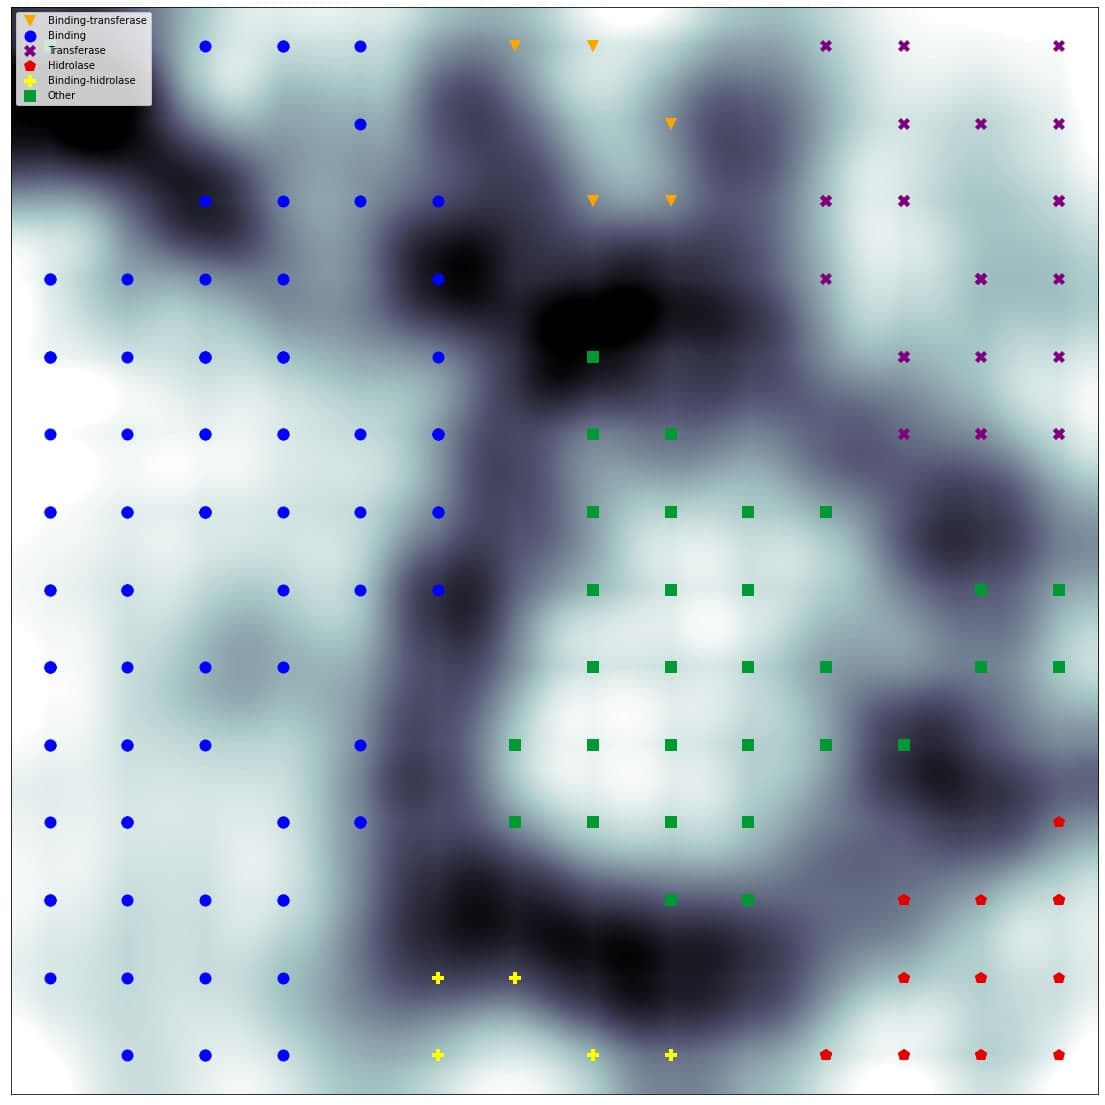
\includegraphics[width=\linewidth]{images/04_SOM.jpg}
	%%\caption{SOM}
	\label{fig:som}
	\endminipage
	\caption{Self organized map of the whole familiome with all of the selected features.
	This map shows the clustered families projected into a 2D space preserving the topology of the data in the original dimension.}
\end{figure}

\clearpage

\begin{figure}[htb]
	\minipage{1.00\textwidth}
	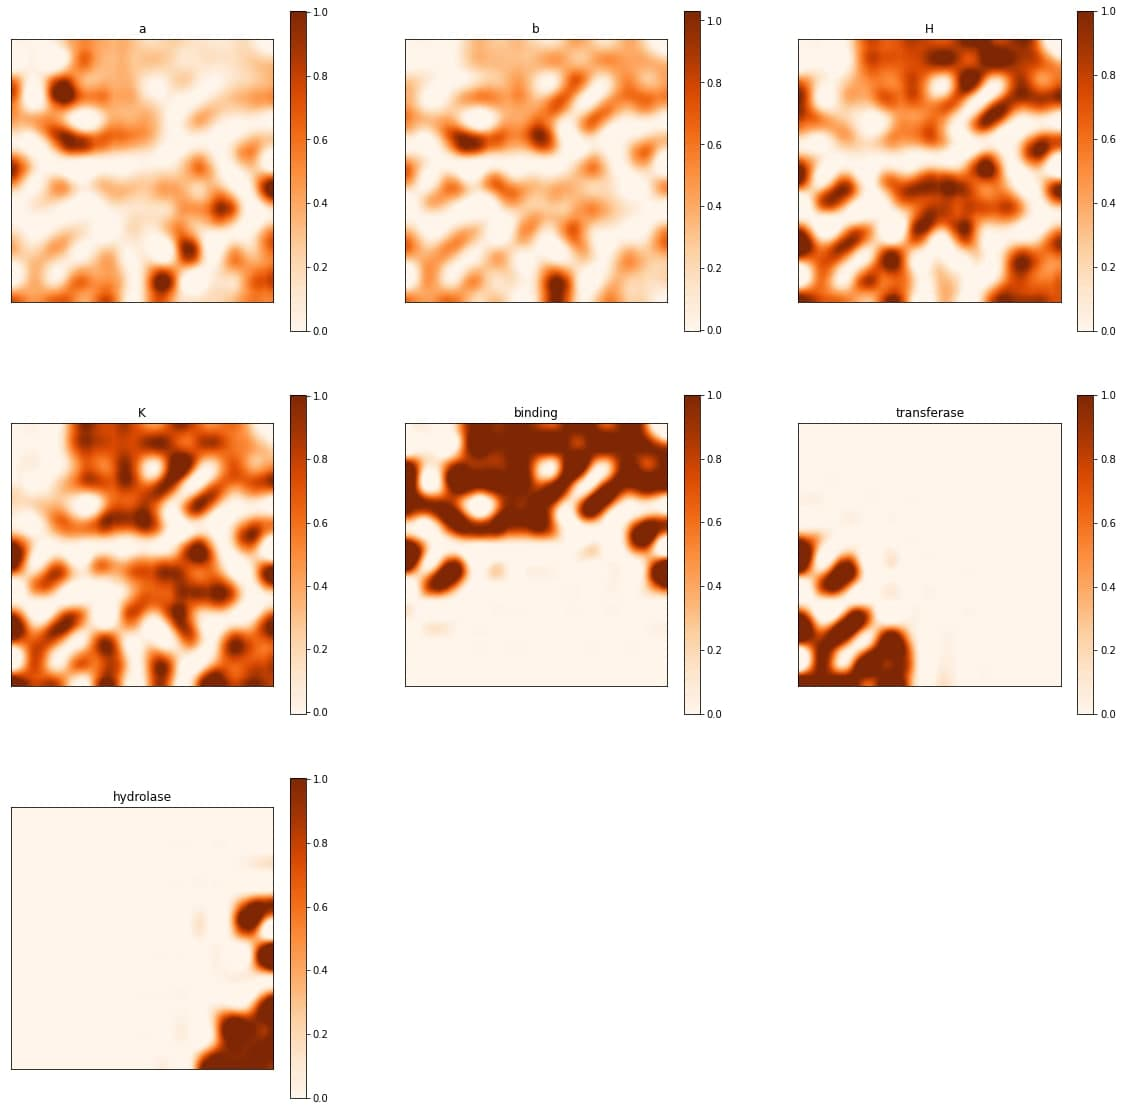
\includegraphics[width=\linewidth]{images/05_SOM.jpg}
	%%\caption{SOM}
	\label{fig:som}
	\endminipage
	\caption{Components of SOM in \label{fig:som}. 
	This figure shows the distribution of the features used to create the SOM which are a is alfa, b is beta, H is Shannon entropy and K is Kolmogorov complexity, 
	the last three are obtained from the gene ontology functions associated with each family}

\end{figure}



Para describir la figura 5.

Qué no se parezcan entre si significa que los componentes son independientes para el SOM y que se parezcan entre si, significa que estadísticamente no son independientes, es decir, que uno dependa del otro. La columna de datos, a y H, b y K dependen estadísticamente entre si. 

\par Poner en algún punto que no se obtuvo la información que se deseaba, o algo así, en cuánto al uso de RIDs/ROs, o simplemente poner que no se sabe cuál es el papel de las RIDs/ROs en esta metodología. 

\clearpage


\section{\textbf{Conclusions.}}
\label{S:1}
NOS INTERESA SABER SI LA GERMIBETA APLICADA A LOS PATRONES DE ORDEN Y DESORDEN DE LAS FAMILIAS DE PROTEÍNAS NOS SIRVE PARA CARACTERIZAR A LAS FAMILIAS DE PROTEÍNAS. SE TIENEN GRÁFICAS EN DÓNDE ESTÁN POR UN LADO LAS RIDS Y LAS ROS EN LA GERMIBETA. 

¿qué significa caracterizar? POR EJEMPLO, SI UNA FAMILIA PERTENECE A UNA FAMILIA O A OTRA, SI EL PATRÓN DE UNA FAMILIA ES CARACTERÍSTICO O ESPECÍFICO PARA CADA UNA DE LAS FAMILIAS O INCLUSO GRUPO DE FAMILIAS, VER SI LA SUMA DE LAS MEDICIONES QUE SE UTILIZARON AGRUPAN A LAS FAMILIAS.
EN DATOS QUE NO SE VAN A PUBLICAR, SE HICIERON SOM's CON DISTINTOS GRUPOS DE DATOS. EN UNO SE UTILIZÓ SOLO EL PARÁMETRO DE LA ONTOLOGÍA Y NO SE OBSERVÓ NINGÚN GRUPO SEPARADO, EN OTRO SOM SOLO SE UTILIZARON LOS DATOS DE KOLMOGOROV, SHANNON Y ONTOLOGÍA Y NO SE OBSERVARON LOS GRUPOS QUE SE TIENEN EN LA FIGURA 4, EN OTRO SOM SE UTILIZARON SOLO LOS DATOS DE LA GERMIBETA Y NO SE OBSERVARON LA SEPARACIÓN DE GRUPOS. COMO CONCLUSIÓN PRELIMINAR, SE PUEDE DECIR QUE LOS CUATROS DATOS SON IMPORTANTES PARA QUE SE AGRUPEN COMO EN LA FIGURA 4. 

EN ALGÚN PUNTO TRATA DE DISCUTIR LO DE LAS REGIONES DESORDENADAS, QUE DEBEN IR DE LA MANO CON LAS REGIONES ORDENADAS, EL TAMAÑO DE LAS REGIONES. DISCUTIR UN POCO SOBRE LA INTEGRACIÓN DE ORDEN/DESORDEN, LAS PROTEÍNAS COEXISTEN ENTRE ESAS DOS REGIONES. LAS RIDs PARA NOSOTROS SON COMO UNA ESPECIE DE HUELLA DIGITAL. 

COMO PERSPECTIVA. QUE SE PUDIERA UTILIZAR EN LA SECUENCIA COMPLETA Y NO SOLO EN DOMINIOS Y EN FAMILIAS PARA LA CREACIÓN DE LA MEGASECUENCIA. 

LA MEDICIÓN DE LA GERMIBETA, KOLMOGOROV Y SHANNON, SON UNA MÉTRICA? SI LA RESPUESTA ES POSITIVA, ENTONCES VALDRÍA LA PENA PONERLO EN LAS CONCLUSIONES. 

EN LA DISCUSIÓN Y LAS CONCLUSIONES "DEBEMOS PONER" EL SIGNIFICADO DE LAS CURVAS, VISUALMENTE HABLANDO?
\bigbreak


\section{\textbf{References.}}
\label{S:1}




%% The Appendices part is started with the command \appendix;
%% appendix sections are then done as normal sections
%% \appendix

%% \section{}
%% \label{}


%% Following citation commands can be used in the body text:
%% Usage of \cite is as follows:
%%   \cite{key}          ==>>  [#]
%%   \cite[chap. 2]{key} ==>>  [#, chap. 2]
%%   \citet{key}         ==>>  Author [#]

%% References with bibTeX database:

% \bibliographystyle{model1-num-names}

%% New version of the num-names style

\bibliographystyle{elsarticle-num-names}
\bibliography{references.bib}

%% Authors are advised to submit their bibtex database files. They are
%% requested to list a bibtex style file in the manuscript if they do
%% not want to use model1-num-names.bst.

%% References without bibTeX database:

% \begin{thebibliography}{00}

%% \bibitem must have the following form:
%%   \bibitem{key}...
%%

% \bibitem{}

% \end{thebibliography}


\end{document}

%%
%% End of file `elsarticle-template-1-num.tex'.
